\documentclass[12pt]{article}
%%%%%%%%%%%%%%%%%%%%%%%%%%%%%%%%%%%%%%%%%%%%%%%%%%%%%%%%%%%%%%%%%%%%%%%%%%%%%%%%%%%%%%%%%%%%%%%%%%%%%%%%%%%%%%%%%%%%%%%%%%%%%%%%%%%%%%%%%%%%%%%%%%%%%%%%%%%%%%%%%%%%%%%%%%%%%%%%%%%%%%%%%%%%%%%%%%%%%%%%%%%%%%%%%%%%%%%%%%%%%%%%%%%%%%%%%%%%%%%%%%%%%%%%%%%%
\usepackage{amsfonts}
\usepackage{eurosym}
\usepackage{geometry}
\usepackage{amsmath,amsthm,amssymb}
\usepackage{ulem} 
\usepackage{graphicx}
\usepackage{comment}
%\usepackage[sort,comma]{natbib}
\usepackage[backend=biber, style = apa]{biblatex}
\usepackage{placeins} % to separate sections

\usepackage{adjustbox}
\usepackage{array}
\usepackage{multirow}
\usepackage{graphicx}
\usepackage{subcaption}
\usepackage{pifont}
\usepackage{amssymb}
\usepackage{comment}
\usepackage[utf8]{inputenc}
\usepackage{setspace}
\usepackage[hang, flushmargin, bottom]{footmisc}
\usepackage{footnotebackref}
\usepackage{xcolor}
\usepackage{hyperref}
\usepackage{booktabs}
\usepackage{pifont}
\usepackage{caption}
\usepackage{float}
\usepackage{todonotes}
\setcounter{MaxMatrixCols}{10}
%TCIDATA{OutputFilter=LATEX.DLL}
%TCIDATA{Version=5.50.0.2960}
%TCIDATA{<META NAME="SaveForMode" CONTENT="1">}
%TCIDATA{BibliographyScheme=BibTeX}
%TCIDATA{LastRevised=Sunday, April 28, 2024 18:12:38}
%TCIDATA{<META NAME="GraphicsSave" CONTENT="32">}
%TCIDATA{Language=American English}

%\setlength{\bibsep}{0.3pt}
\setlength{\textfloatsep}{5pt}
\hypersetup{breaklinks=true,hypertexnames=false,colorlinks=true,citecolor = teal}
\captionsetup{font=normalsize}
\newcommand{\cmark}{\ding{51}}
\def\sym#1{\ifmmode^{#1}\else\(^{#1}\)\fi}
\renewcommand{\thetable}{\Roman{table}}
\geometry{verbose,tmargin=.9in,bmargin=1in,lmargin=.8in,rmargin=.8in,nomarginpar}
\makeatletter
\DeclareTextSymbolDefault{\textquotedbl}{T1}
\theoremstyle{plain}
\newtheorem{thm}{\protect\theoremname}
\theoremstyle{plain}
\newtheorem{prop}[thm]{\protect\propositionname}
\providecommand{\propositionname}{Proposition}
\providecommand{\theoremname}{Theorem}
\makeatother
\providecommand{\propositionname}{Proposition}
\providecommand{\theoremname}{Theorem}
\newtheorem{ass}[thm]{Assumption}
% \input{tcilatex}
\usepackage{tikz}
\usetikzlibrary{shapes.geometric, arrows, positioning}





\addbibresource{references.bib}
\begin{document}




\textbf{Overview}

\begin{itemize}
    \item We present a model of asymmetric competition in insurance markets with selection into  into the market (buyers are sicker on average), but not across firms (identical health mix across insurers).   
    \item Given that there is no selection across firms the average cost is the same for all firms. Despite equal average costs, firms have different marginal costs. 
\end{itemize}


\hline

\medskip

We study an annuities market with private health information and differentiated insurers. Section  \ref{sec:model} presents demand, costs, and equilibrium; Section  \ref{sec:simulation}  uses simulations to quantify how changing the amount of private information affects prices, shares, and costs.


\section{The model}\label{sec:model}
\subsection{Consumer choice}\label{sec:consumer_choice}

Following \textcite[p. 21 and 22]{hortacsu_structural_2023} consider a standard nested logit with two nests:the outside option versus buying an annuity; the inner nest consiste of insurers. 

Denote by $\delta_j$ the mean utility of each option, where $j =0$ represents the outside option. 
Then the probability of choosing insurer $j$ conditional on buying an annuity is 

\begin{equation}\label{eq:inner_prob}
    s_{j\mid A} = \frac{\exp(\delta_{j} / \rho)}{\sum_{k=1}^{J} \exp(\delta_{k} / \rho)}  
\end{equation}
where $\rho \in [0,1]$ measures the degree of independence among the alternatives, if $\rho =1 $ the model is a standard logit (without nests)\footnote{See \href{https://eml.berkeley.edu/choice2/ch4.pdf}{here}.}. 
And the probability of buying an annuity is: 


\begin{equation}\label{eq:outer_nest}
    s_A = \frac{\alpha_A\left(\sum_{j=1}^J \exp(\delta_j/\rho)\right)^\rho }{\alpha_A\left(\sum_{j=1}^J \exp(\delta_j/\rho)\right)^\rho +  \exp \left(\delta_0 \right)}
\end{equation}
Hence, the probability of choosing a particular $j\neq 0$ is: 

\begin{equation}\label{eq:choice_prob}
    s_j = s_{j\mid A} \cdot s_A = 
    \frac{\exp(\delta_{j} / \rho)}{\sum_{k=1}^{J} \exp(\delta_{k} / \rho)}  \cdot \left( \frac{\alpha_A\left(\sum_{j=1}^J \exp(\delta_j/\rho)\right)^\rho }{\alpha_A\left(\sum_{j=1}^J \exp(\delta_j/\rho)\right)^\rho +  \exp \left(\delta_0 \right)}\right)
\end{equation}

Define $h_i$ the health status of buyer $i$, which is private information. Given that $h_i$ affects the expected number of payments when buying the annuity the mean utility of the insurers will depend on it, $\delta_j(h_i)$, where we assume that the mean utility is increasing on the health information. 

Assume that, for any $j\neq 0$,  $\delta_j = f(h_i) + \tilde{\delta}_j$, with $f(\cdot)$ being strictly increasing,  but health status does not affect the outside option. 


Then we have:
\begin{equation}\label{eq:no_selection}
    s_{j\mid A}(h_i) = \frac{\exp((f(h_i) + \tilde{\delta}_j) / \rho)}{\sum_{k=1}^{J} \exp((f(h_i) + \tilde{\delta}_j)/ \rho)} = \frac{\exp( \tilde{\delta}_j / \rho)}{\sum_{k=1}^{J} \exp( \tilde{\delta}_j/ \rho)} \equiv s_{j\mid A}
\end{equation}
implying that, conditional on buying an annuity the health information does not affect the insurer choice. 
 

Moreover 
\begin{align}\label{eq:into_selection}
    s_A(h_i)
    %= \frac{\alpha_A\left(\sum_{j=1}^J \exp((f(h_i) + \tilde{\delta}_j)/\rho)\right)^\rho }{\alpha_A\left(\sum_{j=1}^J \exp((f(h_i) + \tilde{\delta}_j)/\rho)\right)^\rho +  \exp \left(\delta_0 \right)} \\
    = \frac{\alpha_A\exp(f(h_i)/\delta)^\rho\left(\sum_{j=1}^J \exp(\tilde{\delta}_j/\rho)\right)^\rho }{\alpha_A\exp(f(h_i)/\delta)^\rho\left(\sum_{j=1}^J \exp(\tilde{\delta}_j/\rho)\right)^\rho  +  \exp \left(\delta_0 \right)}
\end{align}
implying that the probability of buying an annuity is increasing on health status. 


\subsection{Average and marginal costs}\label{sec:costs}

Define $c_j(h_i)$ the cost for insurer $j$ of selling an annuity to buyer with health status $h_i$, where the cost is increasing on its argument.  Then the average cost of insurer $j$ is\footnote{Remember that we are studying a particular group of the population, hence is the average cost for individuals who have the same observables. }: 

\begin{align}\label{eq:avg_cost}
    \bar{c}_j = \frac{\int c_j(h)\cdot s_j(h) \cdot f_h(h) dh}{\int  s_j(h) \cdot f_h(h) dh}
\end{align}
where $f_h(\cdot)$ is the density of health status. 

The marginal cost is: 
\begin{align}\label{eq:mg_cost}
    c^m_j = \frac{\int c_j(h) \frac{\partial s_j(h)}{\partial p_j}  f_h(h) dh }{\int \frac{\partial s_j(h)}{\partial p_j}  f_h(h) dh }
\end{align}

To obtain a closed form solution for the semi-elasticities we assume  $\tilde{\delta}_j = \hat{\delta}_j - \alpha p_j$. Then: 

\begin{align}\label{eq:price_der}
    \frac{\partial s_j(h)}{\partial p_j} 
    %= -\alpha \ s_j \left[ \left(\frac{1}{\rho}(1-s_{j|A})\right)  + s_{j|A}  (1-s_A) \right]  
    = -\alpha \ s_A(h) s_{j\mid A}(h) \left[ \left(\frac{1}{\rho}(1-s_{j|A}(h))\right)  + s_{j|A}(h)  (1-s_A(h)) \right]  
\end{align}

For the derivation see section \ref{sec:appendix1}.


Note that $\frac{1}{\rho}(1-s_{j|A}(h))$ represents the consumers that are substituting from other firms and $s_{j|A}(h)  (1-s_A(h))$ represents the consumers that are substituting from the outside option. 
If the shocks within the nest are correlated ( $\rho \rightarrow 0 $) then most of the marginal consumers are susbstituting from other firms, whereas if the outside option is very relevant $s_A \rightarrow 1 $ then most of the additional consumers come from the outside option. 


Given that the  probability of buying an annuity is increasing on $h_i$ (see equation \ref{eq:into_selection}), there is adverse selection into the annuities market. The cost of selling an annuity to an annuities buyer is on average higher than the cost of providing an annuity to a buyer choosing the outside option. For a formal proof see section \ref{sec:appendix2}.  

If all firms have the same cost function ($c_j(h) = c(h)$), then the average cost is the same for all firms. We refer by this result as \textit{no selection across firms} since all the cost differences would arise due to different cost functions and not due to consumers sorting into firms. For a formal proof see section \ref{sec:appendix2.1}.

Moreover given that the non-buyers tend to be healthier than the buyers, the marginal cost is lower than the average costs. The intuition is that the marginal cost of a firm is the convex combination of the cost of buyers diverted from other firms and the cost of  buyers diverted from the outside option (see equation \ref{eq:price_der}), where this latter group has a lower cost, whereas the average cost is the same as the cost of buyers diverted from other firms.  For a formal proof that $ \bar{c}_j \geq c_j^m$, see section \ref{sec:appendix3}. 


Even in the case firms have the same cost function, product differentiation generates  heterogeneity in marginal costs. This can appear counterintuitive, because previously we determined that there is no selection across firms which implies that they have the same average costs. To build some intuition, consider a duopoly with market shares 50\%, 1\% and 49\% does not buy the insurance. The market leader, when decreasing the costs, gets the healthy non buyers, whereas the small firms gets a mixture of previous buyers and non-buyers. Hence the bigger firm has smaller marginal costs than the smaller firm. 
For a formal proof see section \ref{sec:appendix3.1}.

\subsection{Firm pricing}\label{sec:pricing}
The firm profits are:

\begin{align}
    \pi_j &= \int ( p_j -c(h) )s_j(h) f(h) dh  
\end{align}

Then the FOC is: 
\begin{align}\label{eq:FOC}
    \int \left[s_j(h)+ ( p_j -c(h) )\frac{\partial s_j(h)}{\partial p_j}\right] f(h) dh =0  \\
    %\int ( p_j -c(h) )\frac{\partial s_j(h)}{\partial p_j} f(h) dh = - \int s_j(h) f(h) dh \notag \\
    %\int  p_j \frac{\partial s_j(h)}{\partial p_j} f(h) dh -  \int c(h) \frac{\partial s_j(h)}{\partial p_j} f(h) dh = - \int s_j(h) f(h) dh \\
    %\int  p_j \frac{\partial s_j(h)}{\partial p_j} f(h) dh - c^m_j \cdot \left(\int \frac{\partial s_j(h)}{\partial p_j}  f(h) dh \right)= - \int s_j(h) f(h) dh \\
    %[ p_j- c^m_j] \int  \frac{\partial s_j(h)}{\partial p_j} f(h) dh = - \int s_j(h) f(h) dh \\
    p_j- c^m_j  = - \frac{\int s_j(h) f(h) dh}{\int  \frac{\partial s_j(h)}{\partial p_j} f(h) dh} = - \frac{ s_j}{\int  \frac{\partial s_j(h)}{\partial p_j} f(h) dh} = \frac{1}{\bar{\eta}_j}
\end{align}
where we used the definition of equation \ref{eq:mg_cost} and we defined $\bar{\eta}_j \equiv -\int \frac{\partial s_j(h)}{\partial p_j}f(j)dh / \int s_j(h) f(h)dh$  the average own-price elasticity. 

As in standard FOC conditions, the margin equals the ratio of market share over a derivative term, but in this particular case the price derivative is the average derivative over health status. 

Using equation \ref{eq:price_der}, and defining the competition weight: 

\begin{align}\label{eq:comp_weight}
    w(h) \equiv s_A(h)s_{j|A}(h)\left[\frac{1}{\rho}(1-s_{j|A}(h)) + s_{j|A}(h)(1-s_A(h))\right]   = -\frac{1}{\alpha} \frac{\partial s_j(h)}{\partial p_j} 
\end{align}

Then we have: 
\begin{align}
    \int \frac{\partial s_j(h)}{\partial p_j} f(h) dh = - \alpha \int w(h) f(h) dh
\end{align}
and the margin can be written as: 
\begin{align}
    p_j- c^m_j  = \frac{ s_j}{\alpha \int w(h) f(h) dh} = 
\end{align}


The higher the market share the higher the margin since raising prices increases profits by increasing revenue from more infra-marginal consumers. 

The higher the competitive pressure the lower the margin, where the competitive pressure is given by the magnitude of marginal consumers. 
For example the smaller the $\rho$ the stronger the correlation of idiosyncratic shocks making competition stronger and decreasing margins.. Or the higher $s_{j\mid A} s_0$ the more likely a consumer switches to the outside option, also decreasing margins. 

Using the FOC and the functional forms previously assumed we can obtain the share of consumers who do not buy an annuity and is given by: 

\begin{align}\label{eq:outside_share2}
    s_0 = \int s_0(h) f_h(h) dh
\end{align}

where: \begin{align}
    s_0(h) = \frac{1}{\alpha_A e^{f(h) -\delta_0}\left[\sum_{j=1}^{J}e^{(\hat{\delta}_j  - \alpha p_j)/\rho}\right]^\rho + 1 } 
\end{align}

For the steps see section \ref{sec:appendix4}. 


\subsection{Effect of increasing information}

In the model we presented, $h_i$ is the private information of the buyer. Providing more information to the sellers implies reducing the role of private information, which we interpret as a decrease in the variance of $h_i$. Assuming that $h_i$ is normally distributed with mean $0$ and standard deviation $\sigma$, we can use our previous results to study the impact of information in various outcomes.

\begin{itemize}
    \item From equation \ref{eq:outside_share2} we can calculate the market share of the outside product and determine what happens when we reduce the role of private information. 

    \item From equations \ref{eq:avg_cost} and \ref{eq:mg_cost} we can calculate the average cost and the marginal cost as a function of $\sigma$ and from them determine the degree of adverse selection. 

\end{itemize}


Note that given that we do not have a close form solution for the equilibrium prices, and as a consequence neither for the market shares and costs, we will perform simulations. In the next section we present the functional forms used and the results obtained. 




\section{Simulation}\label{sec:simulation}

For the simulations we assume that the cost function of the firm is the same for all of them and is given by: 
$c(h) = c_0 + \gamma \cdot h$

Figure \ref{fig:1} shows three patterns. (i) Average cost exceeds marginal cost, consistent with marginal buyers being healthier than the average buyer. (ii) Marginal costs differ across firms even though  $c(\cdot)$ is common. Firms with a higher market share have lower marginal cost.  (iii) Both average and marginal costs rise with $\sigma$. This reflects selection, a higher $\sigma$ increases the share of consumers choosing the outside option, increasing the health status of the marginal consumer. 





\begin{figure}[H]
\caption{}
 \label{fig:1}
\centering{}%
\begin{tabular}{cc}
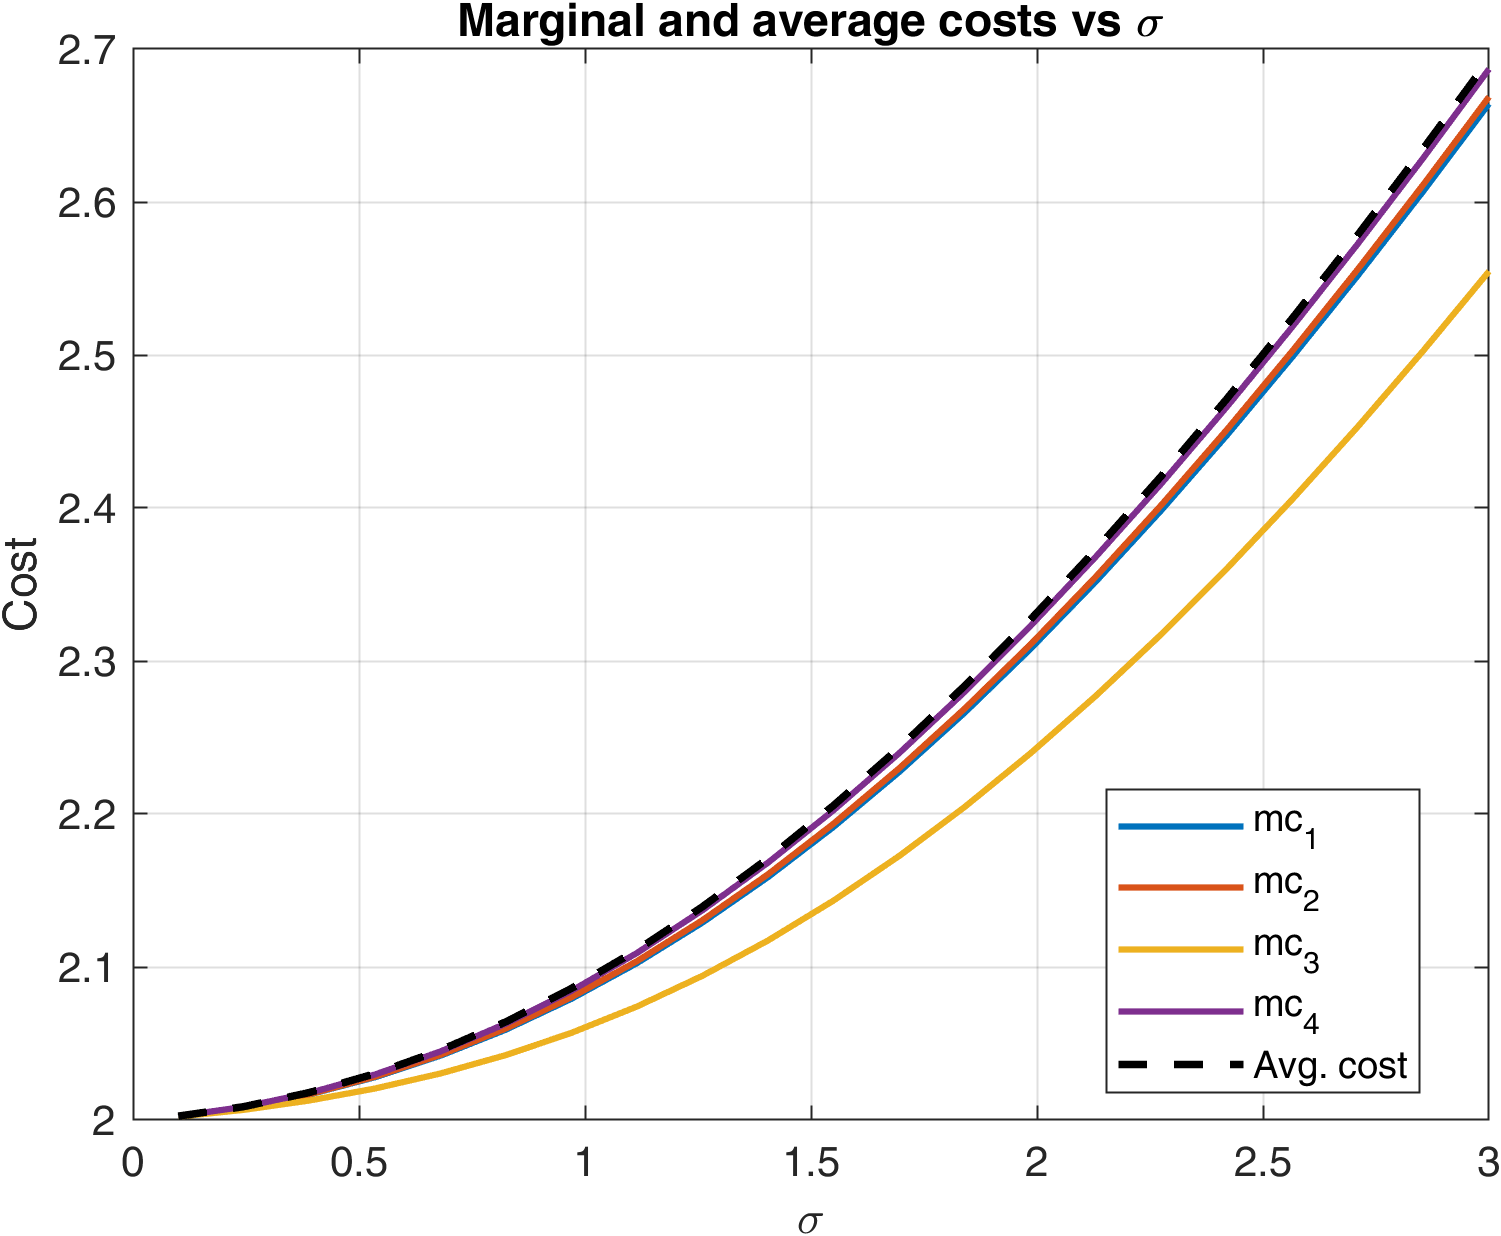
\includegraphics[scale=0.61]{figures/simulations/costs_vs_sigma.png} 
\end{tabular}
\end{figure}


Figure \ref{fig:2} left panel shows the market shares as function of $\sigma$. The main pattern is that when the amount of private information increases (higher $\sigma$) there is unraveling, the amount of individuals choosing the outside option grows. This is generated by higher prices (right panel) which are generated due to the higher level of selection into the market. 


\begin{figure}[H]
\caption{}
 \label{fig:2}
\centering{}%
\begin{tabular}{cc}
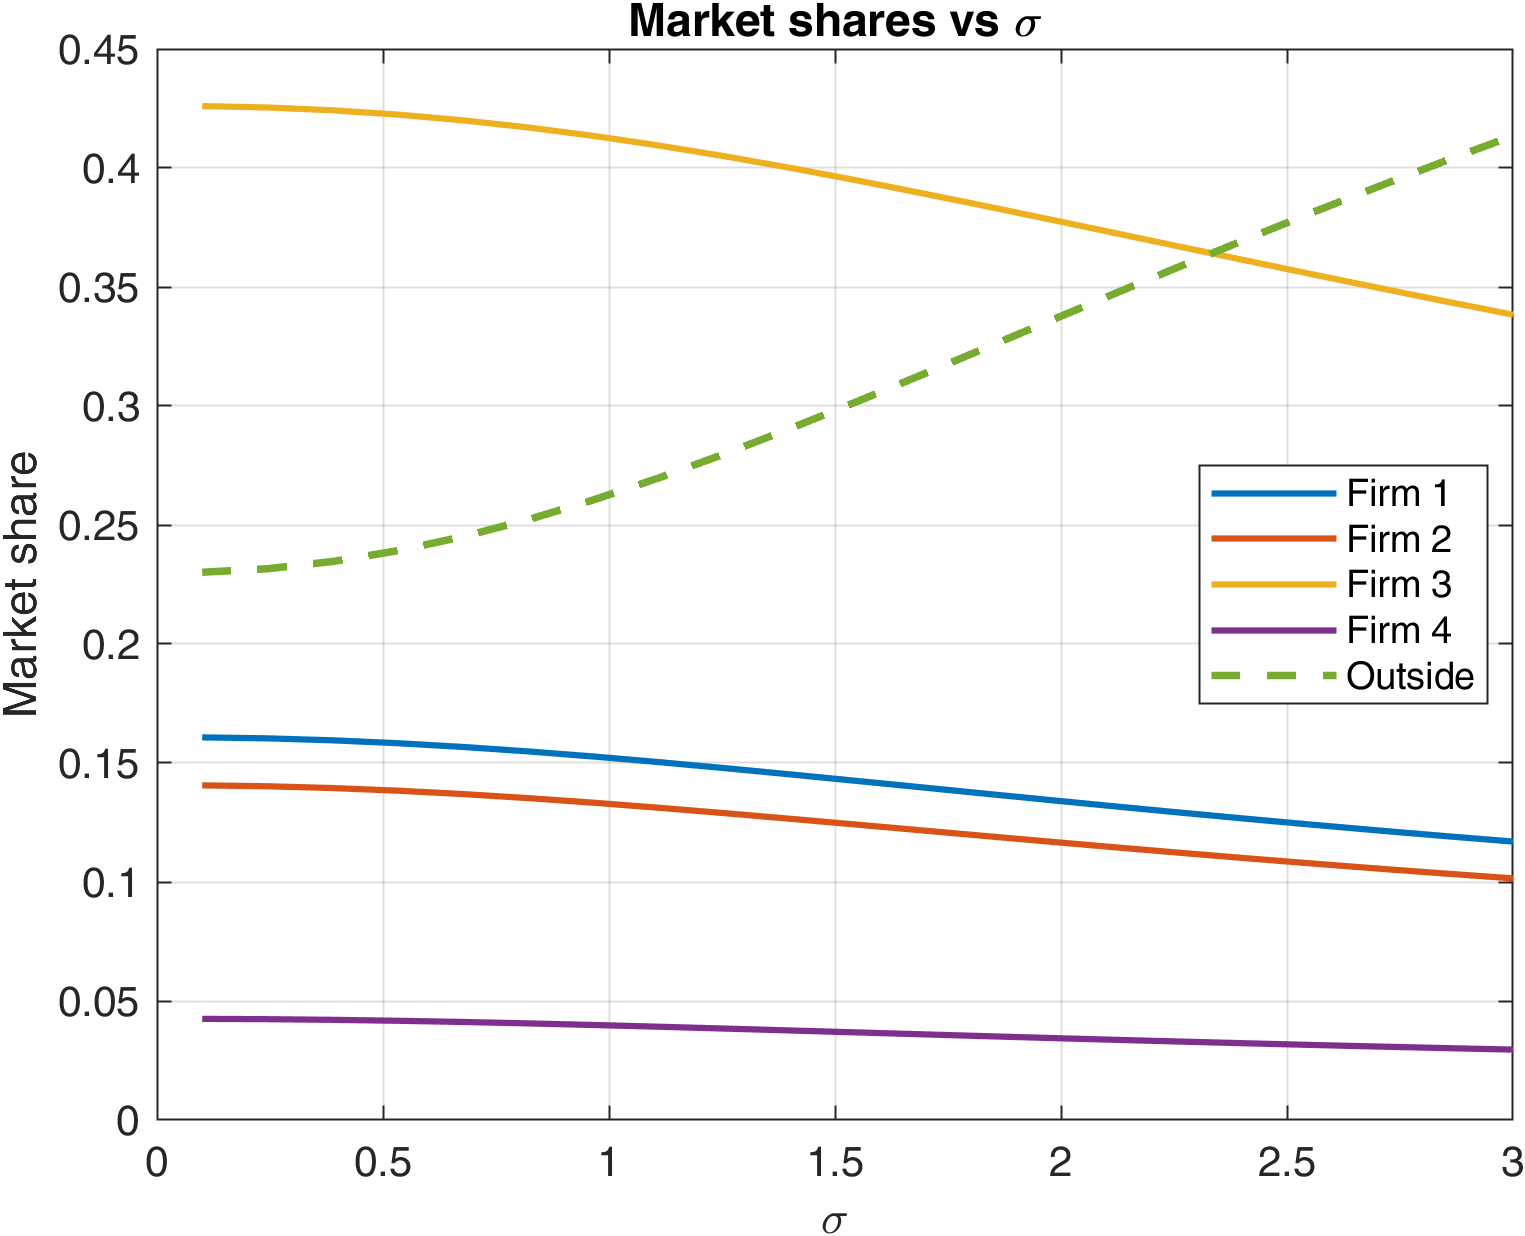
\includegraphics[scale=0.6]{figures/simulations/shares_vs_sigma.png} & 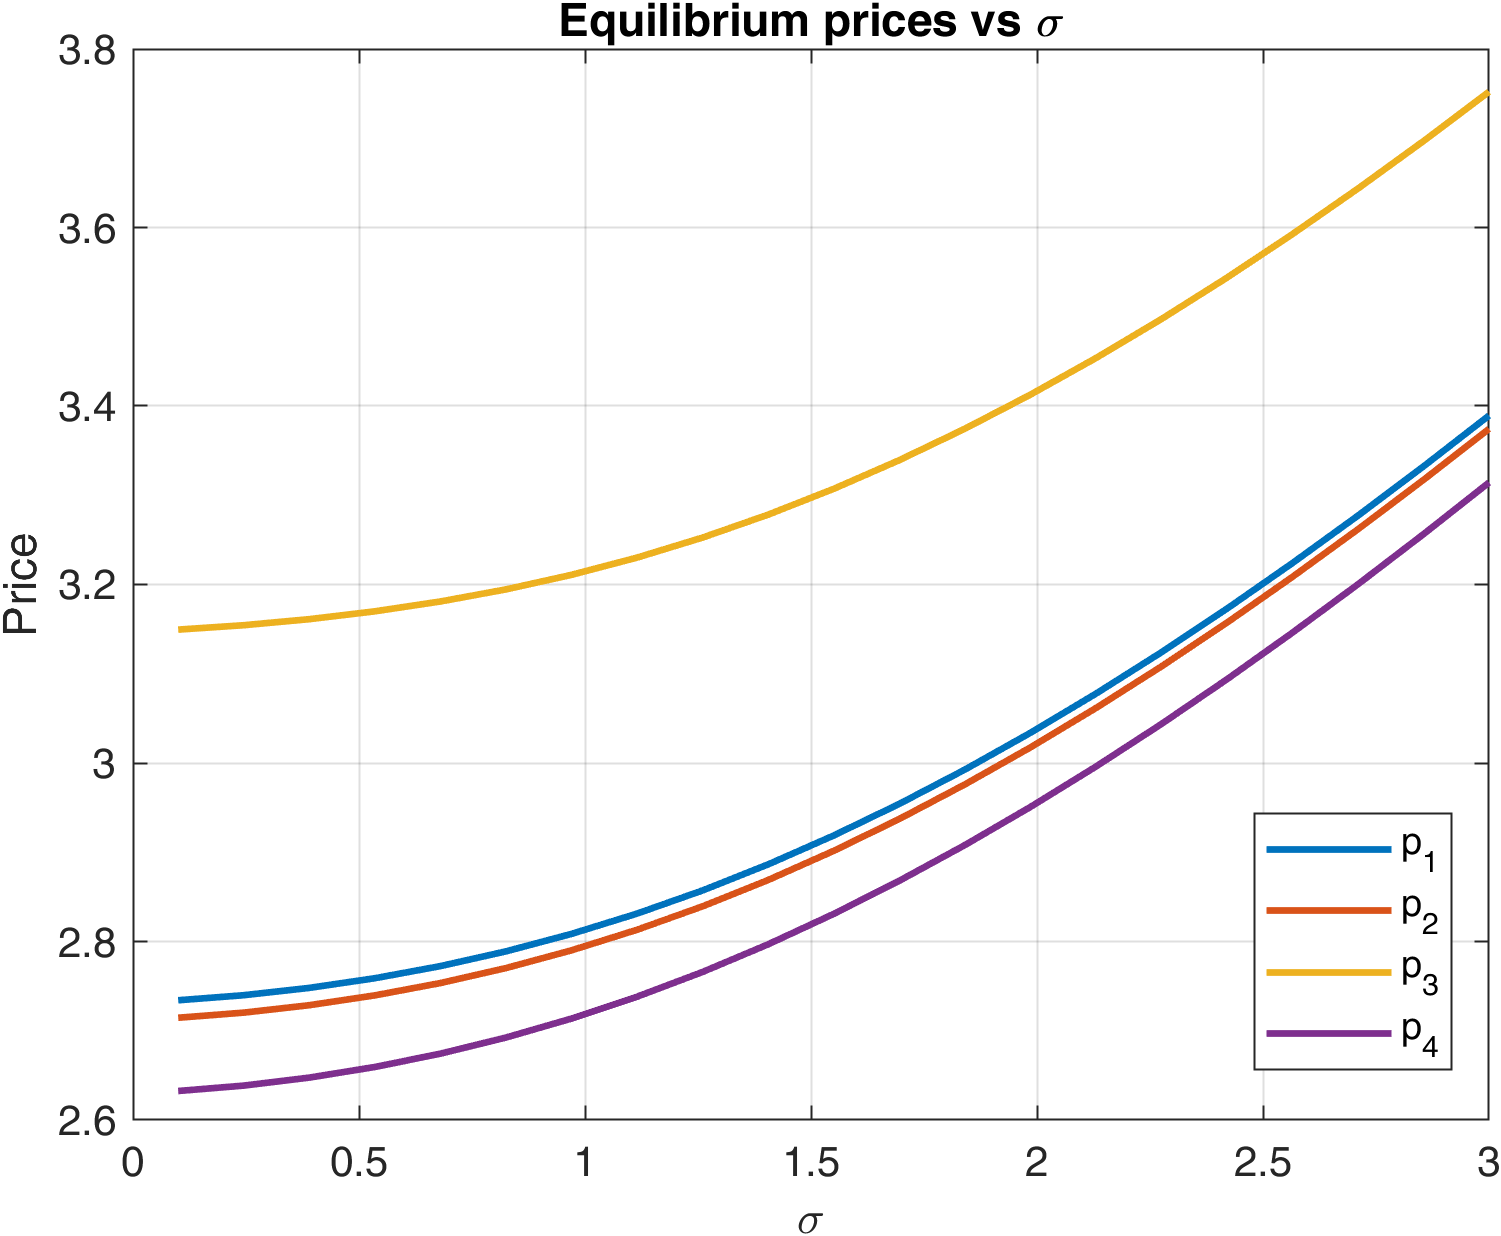
\includegraphics[scale=0.6]{figures/simulations/prices_vs_sigma.png}
\end{tabular}
\end{figure}
\newpage
 

\section{Additional thoughts}

\begin{itemize}
    \item Practitioners told me that the regulator tables are constructed based on the whole population of Chilean retirees, whereas the firms construct their tables based on annuity buyers. From equation \ref{eq:price_der} we can see that in fact the marginal cost is not determined by the mortality of the buyers or non-buyers, but from a combination of both. 

    \item Our model has competition implications. For example a merge will increase market power, but also will decrease the marginal cost beyond just creating synergies, but by increasing the share of marginal buyers who are diverted from the outside option. 
\end{itemize}


\textbf{Effects of firm differentiation}

Consider the case of a homogenous  annuities market, meaning $\delta_j = \delta_A$ for every insurer and $\rho = 0$\footnote{We are not assuming that there are an infinite number of firms.}.
In what follows we compare the homogeneous case with the heterogeneous case. 

Homogeneity affects prices via changing $w(h)$ in two ways. First, given that $\rho \rightarrow 0$, this increases $w(h)$ for any health status. 



From equation \ref{eq:price_der} we can see that the marginal consumer will be diverted from other firms and not from the outside option. 
Given an outside option market share, this will increase costs since the marginal consumer will be healthier.  But of course 


 
\section{Appendix}

\subsection{Own elasticity in nested logit}\label{sec:appendix1}
From equation \ref{eq:choice_prob} we derive the derivative of the probability with respect to price. 

First we have: 

\begin{align}\label{eq:a1}
\frac{\partial s_{j\mid A}}{\partial \delta_j}
%&=\frac{(1/\rho)\cdot e^{\delta_j/\rho}\cdot \sum_{k\in A} e^{\delta_k/\rho}-e^{\delta_j/\rho}\cdot (1/\rho)\cdot e^{\delta_j/\rho}}{\left(\sum_{k\in A} e^{\delta_k/\rho}\right)^2} \\
%&=\frac{1}{\rho}\left(\frac{e^{\delta_j/\rho}}{\sum_{k\in A} e^{\delta_k/\rho}}\right)\frac{  \sum_{k\in A} e^{\delta_k/\rho}-  e^{\delta_j/\rho}}{\sum_{k\in A} e^{\delta_k/\rho}} \\
%&=\frac{1}{\rho}\left(\frac{e^{\delta_j/\rho}}{\sum_{k\in A} e^{\delta_k/\rho}}\right)\left(1-\frac{    e^{\delta_j/\rho}}{\sum_{k\in A} e^{\delta_k/\rho}} \right)\\
&=\frac{1}{\rho}\,s_{j\mid A}\big(1 - s_{j\mid A}\big), 
\end{align}

Define $D= \sum_{k\in A} e^{\delta_k/\rho}$ then $\frac{\partial D}{\partial \delta_j} =\frac{1}{\rho} e^{\delta_j/\rho} $

\begin{align}\label{eq:a2}
\frac{\partial s_A}{\partial \delta_j} &=
\frac{\partial}{\partial \delta_j}\left(\frac{\alpha_A D^\rho}{\alpha_A D^\rho + e^{\delta_0}}  \right) 
= \frac{\alpha_A \rho D^{\rho-1} D' (\alpha_A D^\rho + e^{\delta_0})-\alpha_A \rho D^{\rho-1} D' (\alpha_A D^\rho)}{(\alpha_A D^\rho + e^{\delta_0})^2} \notag \\ 
%=\alpha_A \cdot   \rho  \cdot D^{\rho-1} \cdot D'\frac{   (\alpha_A D^\rho + e^{\delta_0})- (\alpha_A D^\rho)}{(\alpha_A D^\rho + e^{\delta_0})^2}  \\
%=\rho  \cdot D^{-1} \cdot D'\frac{ e^{\delta_0}}{\alpha_A D^\rho + e^{\delta_0}} \frac{\alpha_AD^{\rho}}{\alpha_A D^\rho + e^{\delta_0}} \\
%=\rho  \cdot D^{-1} \cdot D'\frac{ e^{\delta_0}}{\alpha_A D^\rho + e^{\delta_0}} s_A  \\
%= e^{\delta_j/\rho} \cdot D^{-1}  \frac{ e^{\delta_0}}{\alpha_A D^\rho + e^{\delta_0}} s_A  \\
%= s_{j\mid A}  \frac{ e^{\delta_0}}{\alpha_A D^\rho + e^{\delta_0}} s_A  \\
&= s_{j\mid A}  (1-s_A)s_A 
\end{align}


Assuming $\delta_j = u_j - \alpha p_j, $. We can use the chain rule and equations \ref{eq:a1} and \ref{eq:a2} to obtain the derivatives of market shares with respect to prices: 

\begin{align}\label{eq:a3}
     \frac{\partial s_{j|A}}{\partial p_j} = \frac{\partial s_{j|A}}{\partial \delta_j} \cdot \frac{\partial \delta_j}{\partial p_j} = \left(\frac{1}{\rho}s_{j|A}(1-s_{j|A})\right) \cdot (-\alpha) = -\frac{\alpha}{\rho}s_{j|A}(1-s_{j|A})
\end{align}
\begin{align}\label{eq:a4}
    \frac{\partial s_A}{\partial p_j} = \frac{\partial s_A}{\partial \delta_j} \cdot \frac{\partial \delta_j}{\partial p_j} = \frac{\partial s_A}{\partial p_j} = (s_A(1-s_A)s_{j|A}) \cdot (-\alpha) = -\alpha s_A(1-s_A)s_{j|A}    
\end{align}

Finally 
\begin{align}\label{eq:a5}
    \frac{\partial s_j}{\partial p_j} &= \frac{\partial s_{j|A}}{\partial p_j} \cdot s_A + s_{j|A} \cdot \frac{\partial s_A}{\partial p_j} \notag \\
    %&= \left(-\frac{\alpha}{\rho}s_{j|A}(1-s_{j|A})\right) \cdot s_A + s_{j|A} \cdot \left(-\alpha s_A(1-s_A)s_{j|A}\right) \notag \\
    &= -\alpha \cdot s_A \cdot s_{j|A}\left[ \left(\frac{1}{\rho}(1-s_{j|A})\right)  + s_{j|A}  (1-s_A) \right] \notag \\
    &= -\alpha \ s_j \left[ \left(\frac{1}{\rho}(1-s_{j|A})\right)  + s_{j|A}  (1-s_A) \right]  
\end{align}
with a marginal decrease in prices 
note that when decreasing prices the increase due consumers diverting from other insurers is: 

\begin{align}\label{eq:a6}
    \alpha \ s_j  \left(\frac{1}{\rho}(1-s_{j|A})\right)    
\end{align}
and the buyers diverted from the outside option are: 
\begin{align}\label{eq:a7}
    \alpha \ s_j  s_{j|A}  (1-s_A)  
\end{align}

\bigskip


\subsection{Cross elasticity in nested logit}\label{sec:appendix1.1}


Differentiate  equation \ref{eq:choice_prob} with respect to $p_k$: 

\begin{align}\label{eq:app1}
    \frac{\partial s_j}{\partial p_k} = \frac{\partial s_{j|A}}{\partial p_k}s_A + \frac{\partial s_j}{\partial s_A}\frac{\partial s_A}{\partial p_k}, 
\end{align}



Write $D \equiv \sum_{j \in A} e^{\delta_j/\rho}$. Then  $\partial D/\partial\delta_k = (1/\rho)e^{\delta_k/\rho}$. Since $s_{j|A} = e^{\delta_j/\rho}/D$  we have: 

\begin{align}
    \frac{\partial s_{j|A}}{\partial \delta_k} %=  \frac{-(\partial D/\partial\delta_k) e^{\delta_j/\rho}}{D^2} 
    %= \frac{-( (1/\rho)e^{\delta_k/\rho}) e^{\delta_j/\rho}}{D^2} \\
    %=-\frac{1}{\rho} \frac{e^{\delta_k/\rho} e^{\delta_j/\rho}}{D^2} \\
    =-\frac{1}{\rho}s_{j|A}s_{k|A}
\end{align}


For the outer share, from equation \ref{eq:outer_nest} we have: 

\begin{align}
    \frac{\partial s_A}{\partial\delta_k} = s_A(1-s_A)s_{k|A}
\end{align}

Assuming $\delta_k = u_k - \alpha p_k$, we have $\frac{\partial\delta_k}{\partial p_k} = -\alpha$. Thus: 
\begin{align}\label{eq:app4}
    \frac{\partial s_{j|A}}{\partial p_k} = \frac{\partial s_{j|A}}{\partial \delta_k}\frac{\partial \delta_k}{\partial p_k} = \left(-\frac{1}{\rho}s_{j|A}s_{k|A}\right)(-\alpha) = \frac{\alpha}{\rho}s_{j|A}s_{k|A}.
\end{align}

\begin{align}\label{eq:app5}
    \frac{\partial s_A}{\partial p_k} = \frac{\partial s_A}{\partial \delta_k}\frac{\partial \delta_k}{\partial p_k} = (s_A(1-s_A)s_{k|A})(-\alpha) = -\alpha s_A(1-s_A)s_{k|A}    
\end{align}

Pluging equations \ref{eq:app4} and \ref{eq:app5} into \ref{eq:app1} we have: 


\begin{align}\label{eq:app6}
    \frac{\partial s_j}{\partial p_k} 
    %&=\left[\frac{\alpha}{\rho}s_{j|A}s_{k|A}.\right]s_A - s_{j\mid A} \alpha s_A(1-s_A)s_{k|A} \\
    &= \alpha s_A s_{j|A}s_{k|A}\left(\frac{1}{\rho}  - (1-s_A)\right)
\end{align}


\bigskip

\subsection{Cost difference: selection into the market}\label{sec:appendix2}
In this subsection we prove that the average cost for buyers is higher than for non-buyers, what we call selection into the market. 

From equation \ref{eq:into_selection} 
$s_A(h)$ is strictly increasing in $h$.  By Bayes' rule the density among the buyers ($f_A(h)$) and among non-buyers ($f_0(h)$) are: 
    $$f_A(h) = \frac{s_A(h)f(h)}{s_A}, \quad f_0(h) = \frac{(1-s_A(h))f(h)}{s_0}.$$
Consider the likelihood-ratio
    $$R(h) = \frac{f_A(h)}{f_0(h)} = \frac{s_0}{s_A} \cdot \frac{s_A(h)}{1-s_A(h)}.$$

Since $s_A(h)$ is strictly increasing in $h$ then $R(h)$ also is. 
Given that $f_A/f_0$ exhibits the monotone likelihood ratio (MLR) property, then $f_A$ exhibits first order stochastic dominance (FOSD) with respect to $f_0$\footnote{See  \href{https://en.wikipedia.org/wiki/Monotone_likelihood_ratio?utm_source=chatgpt.com}{here}, for a source of the claim that MLR implies FOSD.}. FOSD implies that\footnote{See \href{https://economics.stackexchange.com/questions/15134/implication-of-first-order-stochastic-dominance?utm_source=chatgpt.com}{here} for a proof that FOSD implies an inequality of expected values. }: 

$$E[c(H)|A] \geq E[c(H)|0],$$

\bigskip

\subsection{Cost difference: no across firms selection}\label{sec:appendix2.1}
In this subsection we prove that all firms have the same average cost, there is no selection across firms. 

Assume that $c_j(h) = c(h), \forall j$ then, for any firm $j$: 
\begin{align}
\bar{c}_j = \frac{\int c(h)s_j(h)f(h)\,dh}{\int s_j(h)f(h)\,dh} = \frac{\int c(h)s_A(h) s_{j\mid A}(h)f(h)\,dh}{\int s_A(h) s_{j\mid A}(h)f(h)\,dh} 
=  \frac{\int c(h)s_A(h) f(h)\,dh}{\int s_A(h) f(h)\,dh} = \bar{c}_A    
\end{align}
where the last equality uses equation \ref{eq:no_selection}. 

\bigskip

\subsection{Cost difference: marginal cost lower than average cost}\label{sec:appendix3}



Using equation \ref{eq:price_der} in equation \ref{eq:avg_cost} we have: 
\begin{align}
    c^m_j = \frac{\int c_j(h) \left[\alpha \ s_A(h) s_{j\mid A}(h) \left[ \left(\frac{1}{\rho}(1-s_{j|A}(h))\right)  + s_{j|A}(h)  (1-s_A(h)) \right]  \right]  f_h(h) dh }{\int  \left[\alpha \ s_A(h) s_{j\mid A}(h) \left[ \left(\frac{1}{\rho}(1-s_{j|A}(h))\right)  + s_{j|A}(h)  (1-s_A(h)) \right]  \right]  f_h(h) dh }
\end{align}


using equation \ref{eq:no_selection} we remove the argument of $s_{j\mid A}(h)$: 
\begin{align}
    c^m_j 
    &= \frac{\int c_j(h) \left[\alpha \ s_A(h) s_{j\mid A} \left[ \left(\frac{1}{\rho}(1-s_{j|A})\right)  + s_{j|A}  (1-s_A(h)) \right]  \right]  f_h(h) dh }{\int  \left[\alpha \ s_A(h) s_{j\mid A} \left[ \left(\frac{1}{\rho}(1-s_{j|A})\right)  + s_{j|A}  (1-s_A(h)) \right]  \right]  f_h(h) dh } 
\end{align}
where the numerator is:
\begin{align}\label{eq:numerator}
  \int c_j(h) \left[\alpha \ s_A(h) s_{j\mid A} \frac{1}{\rho}(1-s_{j|A}) \right]  f_h(h) dh +\int c_j(h)\alpha \ s_A(h) s_{j\mid A}  s_{j|A}  (1-s_A(h))  f_h(h) dh \notag \\  
   %= \alpha s_{j\mid A} \frac{1}{\rho}(1-s_{j|A})\int c_j(h)  \ s_A(h) f_h(h) dh +\alpha s_{j\mid A}^2 \int c_j(h) \ s_A(h)    (1-s_A(h))  f_h(h) dh \notag \\  
    = a \int c_j(h)  \ s_A(h) f_h(h) dh +b \int c_j(h) \ s_A(h)    (1-s_A(h))  f_h(h) dh  
\end{align}
where the last step used the definitions $a\equiv  \alpha s_{j\mid A} \frac{1}{\rho}(1-s_{j|A}), \quad b \equiv \alpha s_{j\mid A}^2 $
similarly the  denominator is: 

\begin{align}\label{eq:denominator}
    a \int s_A(h) f_h(h) dh +b \int s_A(h)    (1-s_A(h))  f_h(h) dh  \equiv W
\end{align}
replacing equations \ref{eq:numerator} and \ref{eq:denominator}, we have the marginal cost being: 

\begin{align}\label{eq:mg_cost2}
    c^m_j 
    &= \frac{a \int c_j(h)  \ s_A(h) f_h(h) dh +b \int c_j(h) \ s_A(h)    (1-s_A(h))  f_h(h) dh  }{a \int s_A(h) f_h(h) dh +b \int s_A(h)    (1-s_A(h))  f_h(h) dh }
\end{align}


Define

\begin{align}\label{eq:definitions}
X =   \int c_j(h)  \ s_A(h) f_h(h) dh \quad 
A =   \ s_A(h) f_h(h) dh \notag \\
Y =   \int c_j(h)  \ s_A(h) (1-s_A(h)) f_h(h) dh \quad 
B =   \int s_A(h) (1-s_A(h)) f_h(h) dh 
\end{align}
 replacing in the marginal cost (equation \ref{eq:mg_cost2}) we have: 

 \begin{align}\label{eq:37}
    c^m_j 
    &= \frac{a X +b Y }{aA + bB } = \frac{aA\frac{X}{A}+bB\frac{Y}{B}}{aA+bB} = \frac{aA}{aA+bB}\cdot\frac{X}{A} + \frac{bB}{aA+bB}\cdot\frac{Y}{B}.
\end{align}


Define
$$ \lambda := \frac{aA}{aA+bB} \in [0,1], \quad 1-\lambda = \frac{bB}{aA+bB} \in [0,1].$$

\begin{align}
    c^m_j = \lambda \frac{X}{A} + (1-\lambda)\frac{Y}{B}.
\end{align}

Now we need to prove that $\frac{Y}{B} \le \frac{X}{A}$. 

Introduce the probability measure $d\nu(h) := \frac{s_A(h)f(h)}{A}\,dh$.
Let $r(h) := 1-s_A(h)$. Then
$$E_{\nu}[c_j] = \frac{X}{A}, \quad E_{\nu}[r] = \frac{B}{A}, \quad E_{\nu}[c_j r] = \frac{Y}{A}.$$
Hence
 
$$ \frac{Y}{B} = \frac{E_{\nu}[c_j r]}{E_{\nu}[r]} = \frac{E_{\nu}[c_j]E_{\nu}[r] + Cov_{\nu}(c_j,r)}{E_{\nu}[r]} = E_{\nu}[c_j] + \frac{Cov_{\nu}(c_j,r)}{E_{\nu}[r]} \le E_{\nu}[c_j] = \frac{X}{A},$$
since $c_j$ is (weakly) increasing in $h$ while $r(h)=1-s_A(h)$ is (weakly) decreasing in $h$, implying $Cov_{\nu}(c_j,r) \le 0$. The inequality is strict if both are nonconstant on sets of positive measure.

then we have: 
 \begin{align}
    c^m_j = \lambda \frac{X}{A} + (1-\lambda)\frac{Y}{B} \leq  \lambda \frac{X}{A} + (1-\lambda)\frac{X}{A} = \frac{X}{A} =\bar{c}_j 
\end{align}

\bigskip

\subsection{Cost difference: heterogeneity in marginal costs}\label{sec:appendix3.1}

Using the definitions of equation \ref{eq:definitions} and  $a_j \equiv  \alpha s_{j\mid A} \frac{1}{\rho}(1-s_{j|A}), \quad b_j \equiv \alpha s_{j\mid A}^2 $. 


\begin{align}\label{eq:3.6.1}
W_j & \equiv \alpha \int w_j(h) f(h) dh. = \alpha \int s_A(h) s_{j|A} \left[ \frac{1}{\rho}(1-s_{j|A}) + s_{j|A}(1-s_A(h)) \right] f(h) dh \\
 &= \alpha s_{j|A}\left[ \int s_A(h)   \left[ \frac{1}{\rho}(1-s_{j|A}) + s_{j|A}(1-s_A(h)) \right] f(h) dh \right] \\
&= \alpha s_{j|A} \left[ \frac{1}{\rho}(1-s_{j|A}) \underbrace{\int s_A(h) f(h) dh}_{A} + s_{j|A} \underbrace{\int s_A(h)(1-s_A(h)) f(h) dh}_{B} \right].
\end{align}
where $w_j(h)$ is defined by equation \ref{eq:comp_weight} and $(A,B)$ are defined by equation \ref{eq:definitions}. 

Then we have: 

\begin{equation}
W_j = a_j A + b_j B
\end{equation}

Moreover from equation \ref{eq:37} we have \footnote{In the original equation $a$ and $b$ were not indexed by $j$ just to simplify notation.}:
 \begin{align}
    c^m_j 
    &=  \underbrace{\frac{a_jA}{a_jA+b_jB}}_{\lambda_j}\cdot\frac{X}{A} + \underbrace{\frac{b_jB}{a_jA+b_jB}}_{1-\lambda_j}\cdot\frac{Y}{B}.
\end{align}

Replacing $a_j$ and $b_j$ we have that: 
\begin{align}
    \lambda = \frac{\left(\alpha s_{j\mid A} \frac{1}{\rho}(1-s_{j|A})\right)A}{\left(\alpha s_{j\mid A} \frac{1}{\rho}(1-s_{j|A})\right)A+\left(\alpha s_{j\mid A}^2\right)B}  = \frac{\left(\alpha  \frac{1}{\rho}(1-s_{j|A})\right)A}{\left(\alpha  \frac{1}{\rho}(1-s_{j|A})\right)A+\left(\alpha s_{j\mid A}\right)B} 
\end{align}

note that the differences in marginal cost arise only due to the weights of the linear combination and since  in section \ref{sec:appendix3} we already proved that $ \frac{Y}{B} \leq \frac{X}{A}$, then marginal cost is increasing in  $\lambda_j$. 

This shows that even though the average costs for the firms are the same (see equation \ref{eq:no_selection}), the marginal costs are different. 

Note that 

\begin{align*}
s_{j|A} \to 0 &\implies \lambda_j \to 1 \implies c_{m,j} \to \frac{X}{A}, \\
s_{j|A} \to 1 &\implies \lambda_j \to 0 \implies c_{m,j} \to \frac{Y}{B}.
\end{align*}
Let $u := \frac{1}{\rho}(1-s_{j|A})A$ and $v := s_{j|A}B$, so $\lambda_j = u/(u+v)$. Then
\[
\frac{\partial \lambda_j}{\partial s_{j|A}} = \frac{-\frac{1}{\rho}A(u+v) - u(-\frac{1}{\rho}A+B)}{(u+v)^2} = -\frac{\frac{1}{\rho}Av + uB}{(u+v)^2} < 0, \implies  \frac{\partial c_{m,j}}{\partial s_{j|A}} < 0
\]

Products with \textbf{larger} $s_{j|A}$ have \textbf{smaller} marginal cost. The intution is that products with high market shares get more diversion from the outside margin, where consumers have a lower cost. 

Moreover 
 
\[
\frac{\partial \lambda_j}{\partial \rho} = \frac{(\partial u / \partial \rho)v}{(u+v)^2} = -\frac{(1-s_{j|A})A}{\rho^2} \cdot \frac{v}{(u+v)^2} < 0, \implies  \frac{\partial c_{m,j}}{\partial \rho} < 0 
\]


a \textbf{higher} $\rho$ (weaker within-nest correlation) moves weight toward $\frac{Y}{B}$ and \textbf{lowers} $c_{m,j}$.


   
 

\bigskip

\subsection{Outside share}\label{sec:appendix4}

From equation (\ref{eq:outer_nest}) we have: 

\begin{equation}\label{eq:outside_share}
    s_0(h) = \frac{\exp(\delta_0)}{\alpha_A\left(\sum_{j=1}^J \exp(\delta_j/\rho)\right)^\rho +  \exp \left(\delta_0 \right)}
\end{equation}
Assuming  $\delta_j(h) = f(h) + \bar{\delta}_j$, and defining the within nest inclusive value: 

\[
I_A(h) \equiv \ln \sum_{j=1}^{J} e^{\delta_j(h)/\rho} = \frac{f(h)}{\rho} + \ln \sum_{j=1}^{J} e^{\bar{\delta}_j/\rho}.
\]
Then, replacing in equation \ref{eq:outside_share}, we can write: 


\begin{align}
    s_0(h) %&=\frac{\exp(\delta_0)}{\alpha_A\left(\sum_{j=1}^J \exp(\delta_j/\rho)\right)^\rho +  \exp \left(\delta_0 \right)} \notag \\
    %&= \frac{\exp(\delta_0)}{\alpha_A\left(\exp\{\log(\sum_{j=1}^J \exp(\delta_j/\rho))\}\right)^\rho +  \exp \left(\delta_0 \right)} \notag \\
    %&= \frac{\exp(\delta_0)}{\alpha_A\left(\exp\{I_A(h)\}\right)^\rho +  \exp \left(\delta_0 \right)} \notag \\
    &= \frac{1}{\alpha_A\exp\{I_A(h)\rho - \delta_0\} + 1 } 
\end{align}
replacing the functional form of the inclusive value and parametrizing  $\tilde{\delta}_j = \hat{\delta}_j - \alpha p_j$: 

\begin{align}
    s_0(h) %&= \frac{1}{\alpha_A\exp\{\left[ \frac{f(h)}{\rho} + \ln \sum_{j=1}^{J} e^{\bar{\delta}_j/\rho}\right]\rho - \delta_0\} + 1 } \notag \\
    %&= \frac{1}{\alpha_A\exp\{\left[ f(h) + \rho\ln \sum_{j=1}^{J} e^{\bar{\delta}_j/\rho}\right] - \delta_0\} + 1 } \notag \\
    %&= \frac{1}{\alpha_A e^{f(h) -\delta_0}\exp\{\rho\ln \sum_{j=1}^{J} e^{\bar{\delta}_j/\rho}\} + 1 } \notag \\
    %&= \frac{1}{\alpha_A e^{f(h) -\delta_0}\left[\sum_{j=1}^{J}e^{\bar{\delta}_j/\rho}\right]^\rho + 1 } \notag \\
    &= \frac{1}{\alpha_A e^{f(h) -\delta_0}\left[\sum_{j=1}^{J}e^{(\hat{\delta}_j  - \alpha p_j)/\rho}\right]^\rho + 1 } 
\end{align}


Given the outside share for a given health status we can obtain the outside share in the general popoulation using

\begin{align}
    s_0 = \int s_0(h) f_h(h) dh
\end{align}

 
\end{document}